%# -*- coding: utf-8-unix -*-
% !TEX program = xelatex
% !TEX root = ../thesis.tex
% !TEX encoding = UTF-8 Unicode
%%==================================================
%% chapter01.tex for SJTU Master Thesis
%%第三章
%%==================================================
\chapter{有监督信号的WGAN网络对数据的扩充}
生成式对抗网络(Generative adversarial networks,GAN)\cite{Goodfellow2017NIPS}是深度强化学习应用在数据生成上的成功案例。近年来生成式对抗网络在很多领域有了良好的应用,如:图像合成,图像修补,图像着色,视频预测,文字图像生成,等等。但是生成式对抗网络在其他非图像类领域应用的场景有待发展,其次生成式对抗网络由于损失函数本身是极小极大化的过程,因此纯在训练不稳定,生成样本覆盖不均的缺点。本章将分别介绍原始生成式对抗网络及其发展,并针对特定数据和现有问题提出改进算法原理及方案。
\section{引言}

众所周知,机器学习模型可以根据其学习到的数据形式分为生成式模型(Genenrative Model)和判别式模型(Discriminative Model)。判别式模型是基于决策函数$Y = f(X) $ 或者条件概率分布$ P(Y|X)$进行建模的,判别模型关心的是对于给定的输入$X$ 应该预测出什么样的输出$Y$,输入的数据是原始特征信息,输出的是每条样本对应的标签值。生成式模型由数据学习联合概率分布$P(X,Y)$,然后求条件概率分布$P(Y|X)$作为预测模型,也就是$P(Y|X) = \frac{{P(X,Y)}}{{P(X)}}$,生成式模型可以同时产生样本的特征值及其对应的标签信息\cite{Generative or discriminative? getting the best of both worlds}。典型的判别模型包括:K近邻法\cite{Hartigan1979Algorithm},感知机,决策树,逻辑斯谛回归模型,最大熵模型,支持向量机,提升方法,和条件随机场,等等。在这里我们研究的是小数据集样本的数据扩充,所以用到的是生成式模型,利用极大似然估计算法的深度生成式模型根据其表示或估计似然的方式不同,有很多分类方法\cite{bibid}如图\ref{fig:生成式模型分类树状图}所示。根据似然估计过程基于的函数类型可以将生成模型分为显示密度函数和隐式密度函数,基于显示密度函数的经典算法有PicelRNN\cite{Oord2016Pixel}和变分自编码器\cite{Kingma2013Auto},基于隐式密度函数经典算法有马尔科夫链和生成式对抗网络等等。

\begin{figure}[htpb]
	\centering
	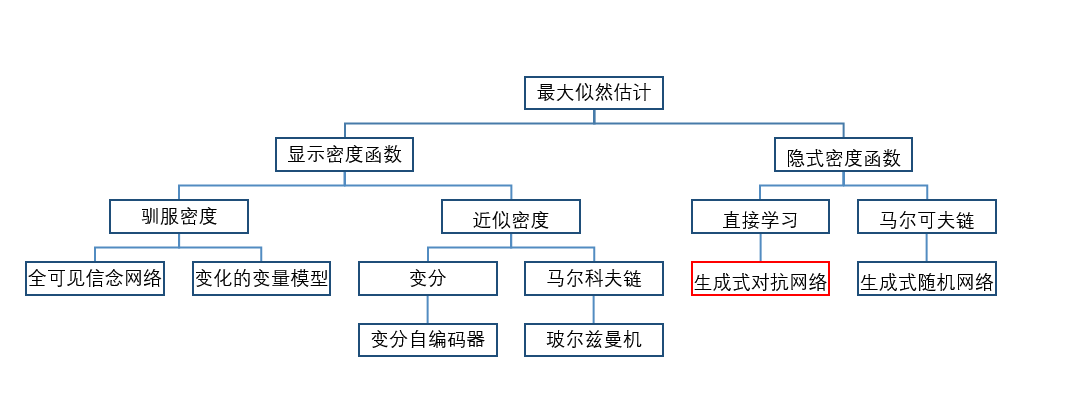
\includegraphics[width=15cm]{example/generate.png}
	\bicaption[这里将出现在插图索引]
	{生成式模型分类树状图}
	{Generated model classification tree graph}
	\label{fig:生成式模型分类树状图}
\end{figure}

在实际问题中,大量样本数据往往很难获得或获取成本较高,而通常情况下在深度学习领域模型又是依赖于大量样本进行学习的,因此对于小样本数据集要想更好的学习数据分布的规律,就需要进行数据增强,在图像领域,常用的数据扩充方法有图像的翻转,旋转,尺度尺度变换,随机抠取,色彩抖动等等,在机器学习领域,常用的方法有Fancy PCA\cite{Holdt2010Genome},监督式抠取,以及我们接下来主要研究的生成式对抗网络的生成方法。数据增强一方面通过增加更多的数据提供信息提高了模型的泛化能力,另一方面引入了更多的噪声数据,能提高模型的鲁棒性。如果数据的分布可以用过模型利用概率统计的方式表达出来,那么产生更多的符合该概率分布的数据就达到了数据增强的目的。本章节主要介绍了生成式对抗网络的基本原理及改进算法,并针对实验数据类型对网络模型引入了监督信息,提高了模型的有效性。
\section{GAN算法}
\subsection{GAN基本框架}
生成式对抗网络于2014年被蒙特利尔大学的Goodfellow Ian首次提出, 由于其出色的表现,引起了业界学者的广泛关注。当强化学习的任务是对样本进行增强时,是通过生成式对抗网络进行实现的。作为Actor-Critic框架下的一员,生成式对抗网络主要有两个部分组成:生成器(Generator)和判别器(Discriminater)。生成器是生成式模型,主要学习数据的联合概率分布,图\ref{fig:生成式模型分类树状图}示意了GAN两个组成部分之间的关系。

\begin{figure}[!htp]
	\centering
	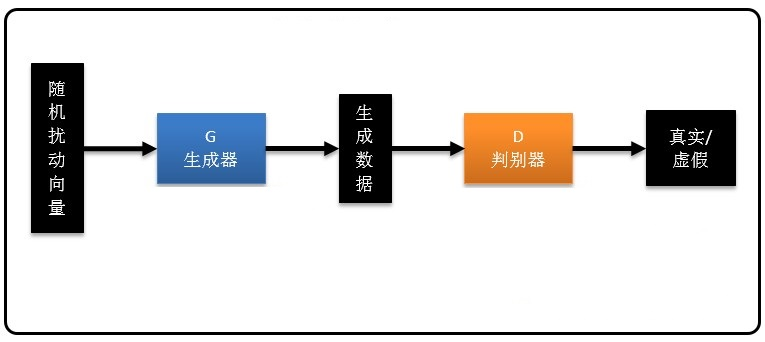
\includegraphics[width=10cm]{example/GAN1.jpg}
	\hspace{1cm}
	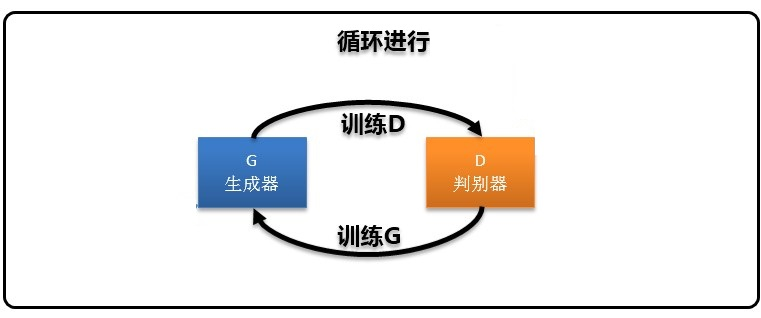
\includegraphics[width=10cm]{example/GAN2.jpg}
	\bicaption[这里将出现在插图索引中]
	{GAN结构示意图}
	{Framework of GAN}
	\label{fig:GAN1}
\end{figure}
其输入的数据为任意形式的噪声,输出的数据为学习到的假样本,判别器相当于一个二分类模型,其输入的数据为原始真实数据和生成器生成的假数据,输出的是输入样本属于真实样本的概率,概率值越大,代表该样本是真实样本的概率越大。生成式利用零和博弈模型把生成式模型和判别式模型整合在了一个框架下。对应于强化学习,GAN里面的生成器相当于智能体,生成器生成的数据就是智能体进行的动作,判别器相当于环境反馈的奖励,当生成的数据越接近真实数据,奖励值越大,生成器会向着该方向更新参数,反之当生成的数据离真实样本分布越远,奖励越小,生成器参数向反方向更新。在这里面,生成器和判别器可以是任何框架下的模型,通常在应用中都使用深层神经网络进行生成器和判别器的构造。

\subsection{GAN算法介绍}
GAN作为生成式模型,求联合概率密度函数离不开极大似然估计,似然估计函数如式\ref{eq:EM}:

\begin{equation}
\label{eq:EM}
\max \limits_{\theta\in R^{d}}\frac{1}{m} \sum_{i=1}^m \log P_{\theta}(x^{(i)})
\end{equation}
在这里,$P_{\theta}$ 是密度函数的参数, $\{x^{(i)}\}^{m} _{i=1}$是从真实数据中采样得到的采样数据。
生成式对抗网络的优化目标函数可以用\ref{eq:22}函数描述。
\begin{equation}
\label{eq:22}
G^{*}=\arg \min \limits_{G} \max \limits_{D} V(G,D)
\end{equation}
这里:
\begin{equation}
\label{eq:33}
V=E_{x\sim P_{data}} [\log D(x)]+E_{x\sim P_{G}}[\log (1-D(x))]
\end{equation}
其中,$P_{data}$代表真实数据的分布,$P_{G}$ 代表生成器学习 $G$得到的假的数据的分布。 $D$ 代表判别器。当我们确定生成器和判别器都是神经网络时,用${\theta _g}$和${\theta _p}$ 分别代表生辰器和判别器的网络结构参数。生成器是可微的。定义输入的噪声数据为$ {p_z}(z)$,可以用${\rm{G(z,}}{\theta _g}{\rm{)}}$表示生成器对数据从噪声分布到学习到数据分布的映射关系。$D(x,{\theta _d})$输出单变量代表概率值。\ref{eq:33}整理为:
\begin{equation}
\label{eq:44}
\mathop {\min }\limits_G \mathop {\max }\limits_D v(D,G) = {E_{x \sim {p_{data}}(x)}}[\log D(x)] + {E_{z \sim {p_z}(z)}}[\log (1 - D(G(z)))]
\end{equation}
 这是一个极小极大化的损失函数,对于一个固定的$G$,对$D$求解其最优函数:
 \begin{equation}
 \label{eq:34}
 {D^*}(x) = \frac{{{p_{data}}(x)}}{{{p_{data}}(x) + {p_g}(x)}}
\end{equation}
 类似地,对于固定的$G$,求$D$的目标是最大化损失函数
\begin{equation}\label{eq:36}
\begin{split}
v(G,D) =& \int_x {{p_{data}}(x)\log (D(x))}\mathrm{d}x + \int_z {{p_z}(z)\log (D(z))}\mathrm{d}x  \\
=&  \int_x \bigg( {{p_{data}}\log ({\rm{D}}(x)) + {p_g}(x)\log (1 - D(x))\bigg)}\mathrm{d}x 
\end{split}
\end{equation}
所以\ref{eq:33},\ref{eq:22}可以整理为:
\begin{equation}
\label{eq:35}
\begin{split}
\mathop {\max }\limits_D v(G,D) =& {E_{x \sim {p_{data}}}}[\log {D^*}_G(x)] + {E_{x \sim {p_g}}}[\log (1 - {D^*}_G(x))] \\
=& {E_{x \sim {p_{data}}}}[\log \frac{{{p_{data}}(x)}}{{{p_{data}}(x) + {p_g}(x)}}] + {E_{x \sim {p_g}}}[\log \frac{{{p_{data}}(x)}}{{{p_{data}}(x) + {p_g}(x)}}]
\end{split}
\end{equation}
整理后得到:
\begin{equation}
\label{eq:37}
\mathop {\max }\limits_D v(G,D) =  - \log 4 + KL({p_{data}}||\frac{{{p_{data}} + {p_g}}}{2}) + KL({p_g}||\frac{{{p_{data}} + {p_g}}}{2})
\end{equation}
其中$KL$ 项表示$KL$散度\cite{joyce2011kullback},是衡量两个数据分布之间距离的函数。整理成$ JS $ 散度衡量变成:
\begin{equation}
\label{eq:38}
\mathop {\max }\limits_D v(G,D) =  - \log 4 + 2JSD({p_{data}}||{p_g})
\end{equation}

可以证明当生成器和判别器的有足够的泛化拟合能力时,对于固定的生成器,判别器都可以达到最优,然后最大化$\mathop {\max }\limits_D v(G,D) = {E_{x \sim {p_{data}}}}[\log {D^*}_G(x)] + {E_{x \sim {p_g}}}[\log (1 - {D^*}_G(x))]$ 求最优的生成器。最后$P_g$将收敛于$p_data$。这样,损失函数可以理解为判别器希望生成的假数据和原始数据分布之间的距离越大越好,而生成器希望两个数据之间的分布越接近越好。GAN训练过程的示意图如\ref{fig:train}所示。

\begin{figure}[htpb]
	\centering
	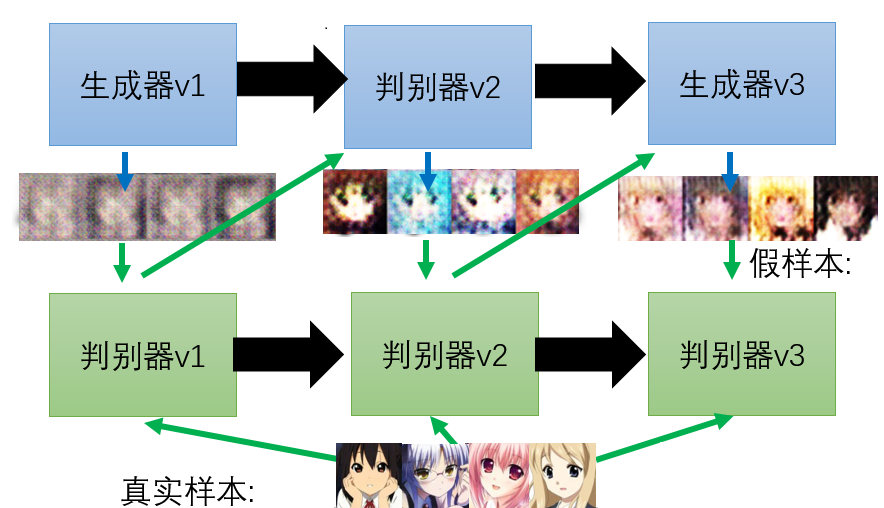
\includegraphics[width=15cm]{example/GAN3.png}
	\bicaption[这里将出现在插图索引]
	{GAN训练过程图示}
	{Generated model classification tree graph}
	\label{fig:train}
\end{figure}

先随机初始化生成器和判别器参数,生成器$v1$生成初始版本假数据连同真实数据一起作为判别器$V1$的输入,判别器$v1$把判别结果送给$v2$生成器,给$v2$生成器打分指导其参数更新的方向。然后$v2$生成器生成新的一批假数据,在这里给真实数据打标签为1,假数据打标签为0,两种数据一起作为判别器$v2$训练的样本数据,循环以上过程,直到整个网络达到一个相对稳定的状态。
算法描述如下:

\begin{algorithm}[!h]
	\caption{GAN 算法}% Ëã·¨±êÌâ
	\begin{algorithmic}[1]%Ò»ÐÐÒ»¸ö±êÐкÅ
		%\Require {The number of critic iterations per generator iteration $n_{critic}$,the batch size $m$, training iteration is $K$.}
		%\Require ~~ \\
		\Require
		对于生成器每次更新,判别器更新的次数$n_{critic}$,批训练样本大小$m$,训练迭代次数为 $K$
		\For{$t=1$ to $K$}
		\For{$i=1$ to $n_{critic}$}
		\State 从噪声数据$Z$中采样$m$个数据:${z^{(1)},...,z^{(m)}}$
		\State
		从真实数据$X$中采样$m$个数据:${x^{(1)},...,x^{(m)}}$ 
		\State 利用随机梯度上升法更新判别器网络参数:
		\begin{equation*}
			{\nabla _{{\theta _{\rm{d}}}}}\frac{{\rm{1}}}{m}\sum\limits_{i = 1}^m {[\log D({x^{(i)}}) + \log (1 - D(G({z^{(i)}})))]} 
		\end{equation*}
		\EndFor
		\State 从噪声数据$Z$中采样$m$个数据:${z^{(1)},...,z^{(m)}}$
		\State
		从真实数据$X$中采样$m$个数据:${x^{(1)},...,x^{(m)}}$ 
		\State 利用随机梯度下降法更新生成器网络参数:
		\begin{equation*}
		{\nabla _{{\theta _g}}}\frac{{\rm{1}}}{m}\sum\limits_{i = 1}^m {\log (1 - D(G({z^{(i)}})))}
		\end{equation*}
		\EndFor
	\end{algorithmic}
\end{algorithm}

\section{WGAN算法}
由于原始的GAN算法存在以下三个难以解决的问题\cite{12}:
\begin{enumerate}
	\item 模式崩溃(Mode collapse),也是GAN算法最大的不足。模式崩溃指生成器更倾向于生成具有较高概率密度的数据,对于出现次数较少的数据生成器缺少对其学习表征的能力。因此导致模型生成的数据过于单一不能完整覆盖到所有样本集。
	\item 梯度消失问题。是指由于判别器学习的速度大于生成器,因此很容易区分真假数据,经过神经网络的层层传递导致梯度消失或爆炸,导致网络无法正常更新。
	\item 无法实时的评价生成数据的质量。这是由于衡量数据分布的函数是JS散度,当两组数据在空间中完全不相交时,JS散度为定值,不能直接反映出两个数据的接近程度。
\end{enumerate}
针对以上问题,WGAN\cite{arjovsky2017wasserstein}算法提出了以下两点改进:
\begin{enumerate}
\item  利用Wasserstein距离(Earth-Mover (EM) distance or Wasserstein distance )代替原来的JS散度来衡量两个数据分布的距离。
\item 为了满足判别器符合一阶利普西茨(1-Lipschtiz)条件,对两组数据连线的中点进行采样。
\end{enumerate}

Wasserstein距离的定义如下:

\begin{equation}
\label{eq37}
W(P_{data},P_{G})= \inf \limits_{\gamma \sim \prod (P_{data},P_{G})} E_{(x,y)\sim\gamma}[\mid\mid x-y\mid\mid]
\end{equation}
其中${ \prod (P_{data},P_{G})}$代表所有以 $P_{data}$ 为 $P_{G}$为边缘概率分布的联合分布$\gamma(x,y)$ 的集合。Wasserstein距离直观意义是数据从一个分布变成另一个分布所需要的最小代价,当数据分布的支撑集位于低维流形,在这里Wasserstein距离是处处连续可导的,Wasserstein距离要优于JS散度或者KL散度,这是因为后者或大或小,而前者始终是平滑的。根据Kantorovich-Rubinstein对偶性,式\ref{eq37}整理为:
\begin{equation}
\label{eq38}
W(P_{data},P_{G})= \frac{1}{K} \sup \limits_{\| f \| _{L} \leq K} E_{x\sim P_{data}}[f(x)]-E_{x\sim P_{G}}[f(x)]
\end{equation}
WGAN优化的损失函数为:
\begin{equation}
\label{eq39}
V= \max \limits_{D\in 1- Lipschitz} E_{x\sim P_{data}}[D(x)]-E_{x\sim P_{G}}[D(x)]
\end{equation}
这里 $D$ 是满足一阶利普西茨条件的函数,可以看出来WGAN相对于GAN算法去掉了原来的log函数,从机器学习的角度可以解释为把原来网络结构的sigmoid函数去掉并加上了利普西茨限制条件。为了满足一阶利普西茨条件,目标函数可以用以下公式表达:
\begin{equation}
\label{eq10}
\begin{aligned}
L=&\mathop{E}_{\tilde{x} \sim P_{G}}[D( \tilde{x})]- \mathop{E}_{x \sim P_{data}}[D(x)]+ \\&\lambda \mathop{E}_{\hat{x}\sim P_{ {penalty}}} [(\| \nabla _{  \hat{x}} D(\hat{x}) \|_{2} - 1)^{2}]
\end{aligned}
\end{equation}

在这里,$\hat{x}\sim P_{ {penalty}}$被定义为从真假数据各随机采样一个数据,他们之间连线的中点所构成的数据分布。这种利用penalty方法的WGAN成为提升WGAN(Improved WGAN)用Wasserstein距离的好处是无论生成数据和原始数据是否有相交部分,判别器都能持续给生成器提供梯度。此外,WGAN另一个显著优势是,其值函数与生成数据分布与原始数据分布之间的差异直接相关,而GAN并非如此。
图\ref{fig:train}展示了提升WGAN相对于传统的DCGAN,LSGAN,WGAN 在图像生成上取得的效果对比。在这里生成器和判别器可以用全连接层,也可以用CNN。可以看出在没有经过批归一化的网络或者没有经过适当调参的网络上提升WGAN表现要好于其他三种算法。因此WGAN相对而言要容易收敛。
\begin{figure}[!htp]
	\centering
	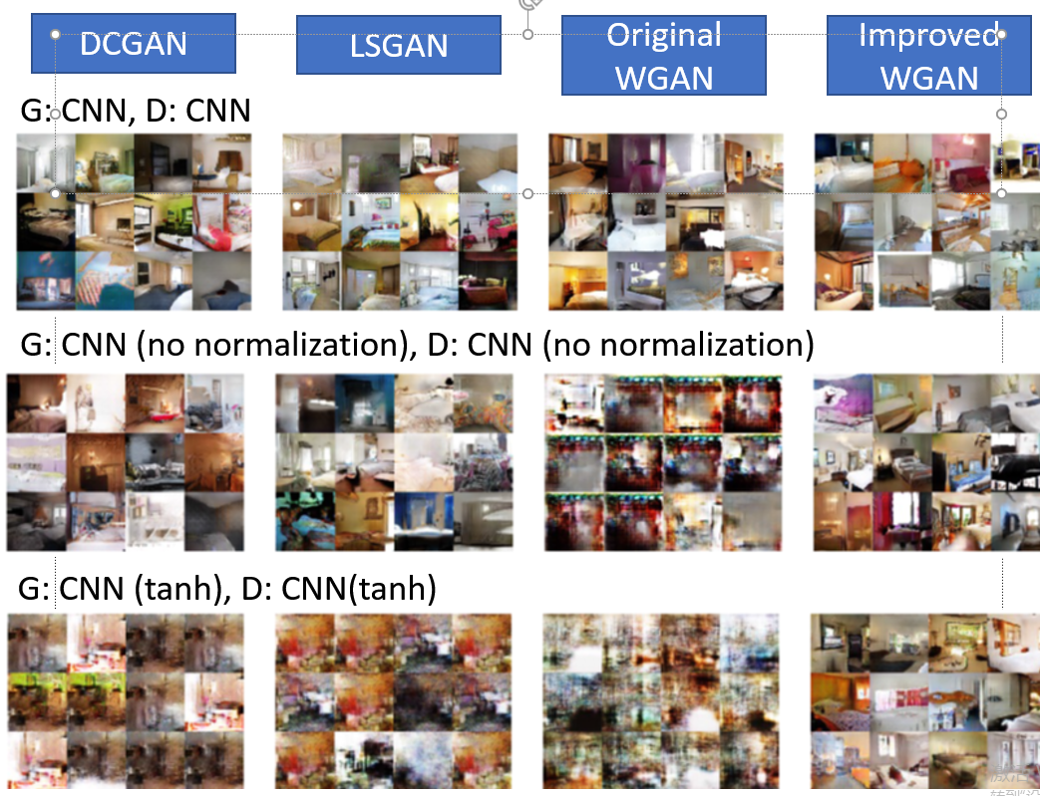
\includegraphics[width=10cm]{example/WGAN1.jpg}
	\hspace{1cm}
%	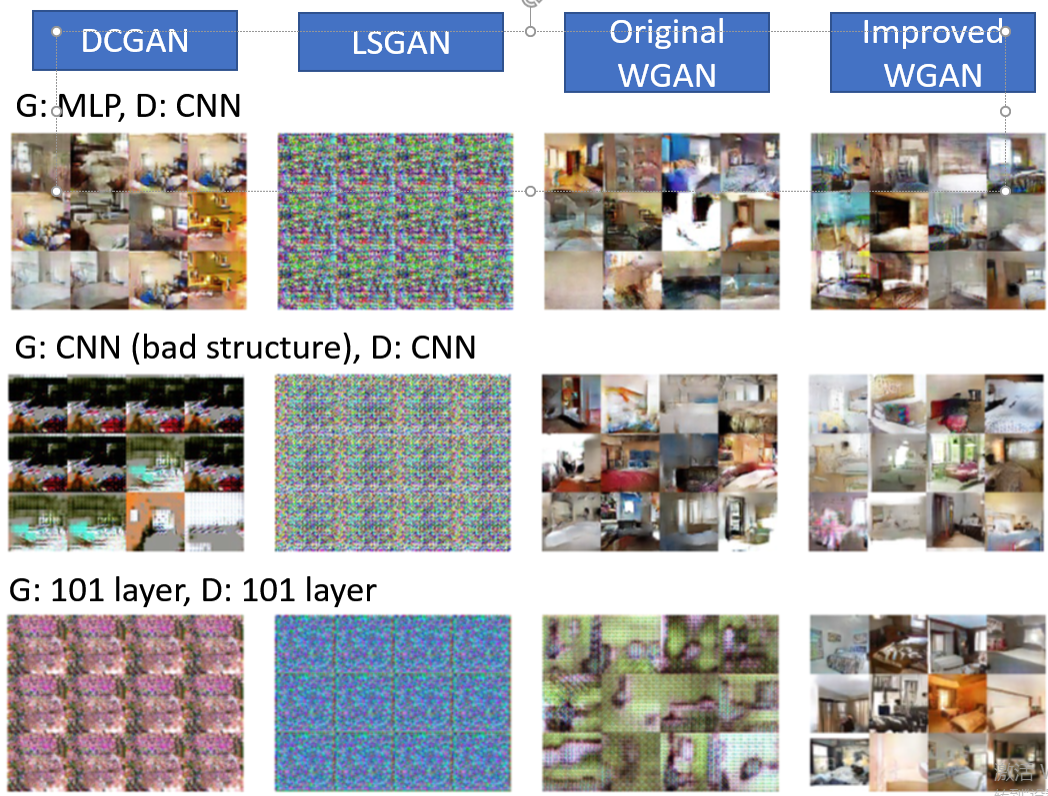
\includegraphics[width=10cm]{example/WGAN2.png}
	\bicaption[这里将出现在插图索引中]
	{GAN结构示意图}
	{Framework of GAN}
	\label{fig:GAN1}
\end{figure}

\section{改进的有监督信号的WGAN算法}
如前面内容提到的,GAN现在主要应用于图像视频领域,对于非图像类数据还没有良好的应用效果。在这一节,将详细介绍改进的WGAN算法。WGAN主要结合了自动编码机(Auto-Encoder,AE)模型学习隐向量的表征能力和WGAN提供持续梯度的优势。通过自动编码机模型引入监督信号,把原来没有监督信息的生成模型变成了利用重构误差衡量其模型好坏的方案。
\subsection{引入监督信息}
监督学习模型因为其优化的目标函数具有规则的几何形状,所以可以有效解决模型梯度消失的问题。\cite{11}。真实的样本可以通过输入隐式空间向量来重建一个性能良好的模型,这样就给生成模型提供了有监督的信号。也就是说,GAN中的生成器可以作为解码器把经过自动编码机编码后的隐向量进行解码操作,把压缩后的特征还原到原始特征空间$X$。在这种有监督的训练过程中,隐向量可以看作是低维空间$Z$中固定的先验分布。因此,先验知识由AE获得,这种方法在机器学习领域的编码工作中得到了广泛的应用。与VAE相比,AE没有额外的隐向量分布的限制。监督信号的优化目标可以描述为:  $ G(E(X))\rightarrow X $。最优的生成器可以最小化$ G(E(X))$和$X$之间的差异。在随机噪声数据的输入中加入规则信息,避免了大量的盲试过程。能够加快模型的收敛速度,提升模型的学习能力。
\subsection{变分GAN}
VAEGAN将在GAN鉴别器中学习到的特征表示作为VAE的基础。其结合方式如图\ref{figVAEGAN}所示。

\begin{figure}[!htp]
	\centering
	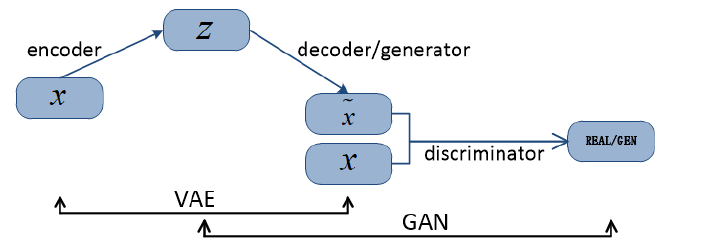
\includegraphics[width=\hsize]{example/VAEGAN.png}
	\bicaption[这里将出现在插图索引]
	{VAEGAN 结构示意图}
	{The Structure Diagram of VAEGAN}
	\label{figVAEGAN}
\end{figure}

与原始的VAE相比,VAEGANs将元素误差替换为特征误差,以更好地捕获数据分布,同时提供不变量\cite{7}。VAE的理论是概率变分界\cite{16},即:

\begin{equation}
\label{eq18}
p(x)\geq E_{q(x\mid z)}[log p (x\mid z)]- KL(q(z\mid x)\parallel P (z))
\end{equation}

然而,由于VAE的结构,VAEGAN不得不遵循这样的假设:潜在变量可以通过分解高斯分布很好地拟合,而高斯分布只有一种模式。在上述约束条件下,编码器将实际样本转化为潜在空间,使生成的潜在向量大致服从正态分布。编码器的输出是加到高斯噪声中的隐藏变量的均值和方差。VAEGAN的解码器与GAN的鉴别器具有相同的参数,即原始VAE的解码器被GAN的鉴别器所替代,这样做的好处是可以更好的了解潜在的特征。

VAEGAN使用GAN的鉴别器作为一种学习相似性度量,但没有利用GAN强大的生成能力。在数据的重构和修复上有很好的效果,但是在数据增强表现一般。VAE是基于潜伏期向量可以近似为高斯分布的假设。然而,对于单模态下不能拟合出潜在空间的GAN,这种假设是不必要的。

虽然WGAN解决了梯度消失的问题,并提供了生成样本的直接评价准则,但是没有对象能够保证遍历所有模式的样本。模态崩溃仍然是一个主要问题。发生器的输入是高斯噪声,其随机性导致训练过程不稳定,收敛缓慢\cite{17}等问题,这种现象在训练初期尤为明显。

到目前为止,所有的VAEGAN和WGAN实验都是基于CIFAR-10、LSUN睡房数据集和MNIST等图像数据,取得了显著的效果。GAN的应用领域还没有扩展到非图像的机器学习领域。

\subsection{改进的WGAN算法描述}
改进的WGAN的具体实现过程为:
除了高斯噪声,隐式特征向量也一起作为输入数据传给生成器,作为数据生成的额外附加信息,隐向量携带着数据本身的一些信息。将AE与WGAN相结合,可以在编码器中使用学习到的特征表示作为WGAN生成目标的基础。改进算法的框架如图~\ref{fig2}所示。

\begin{figure}[!htp]
	\centering
	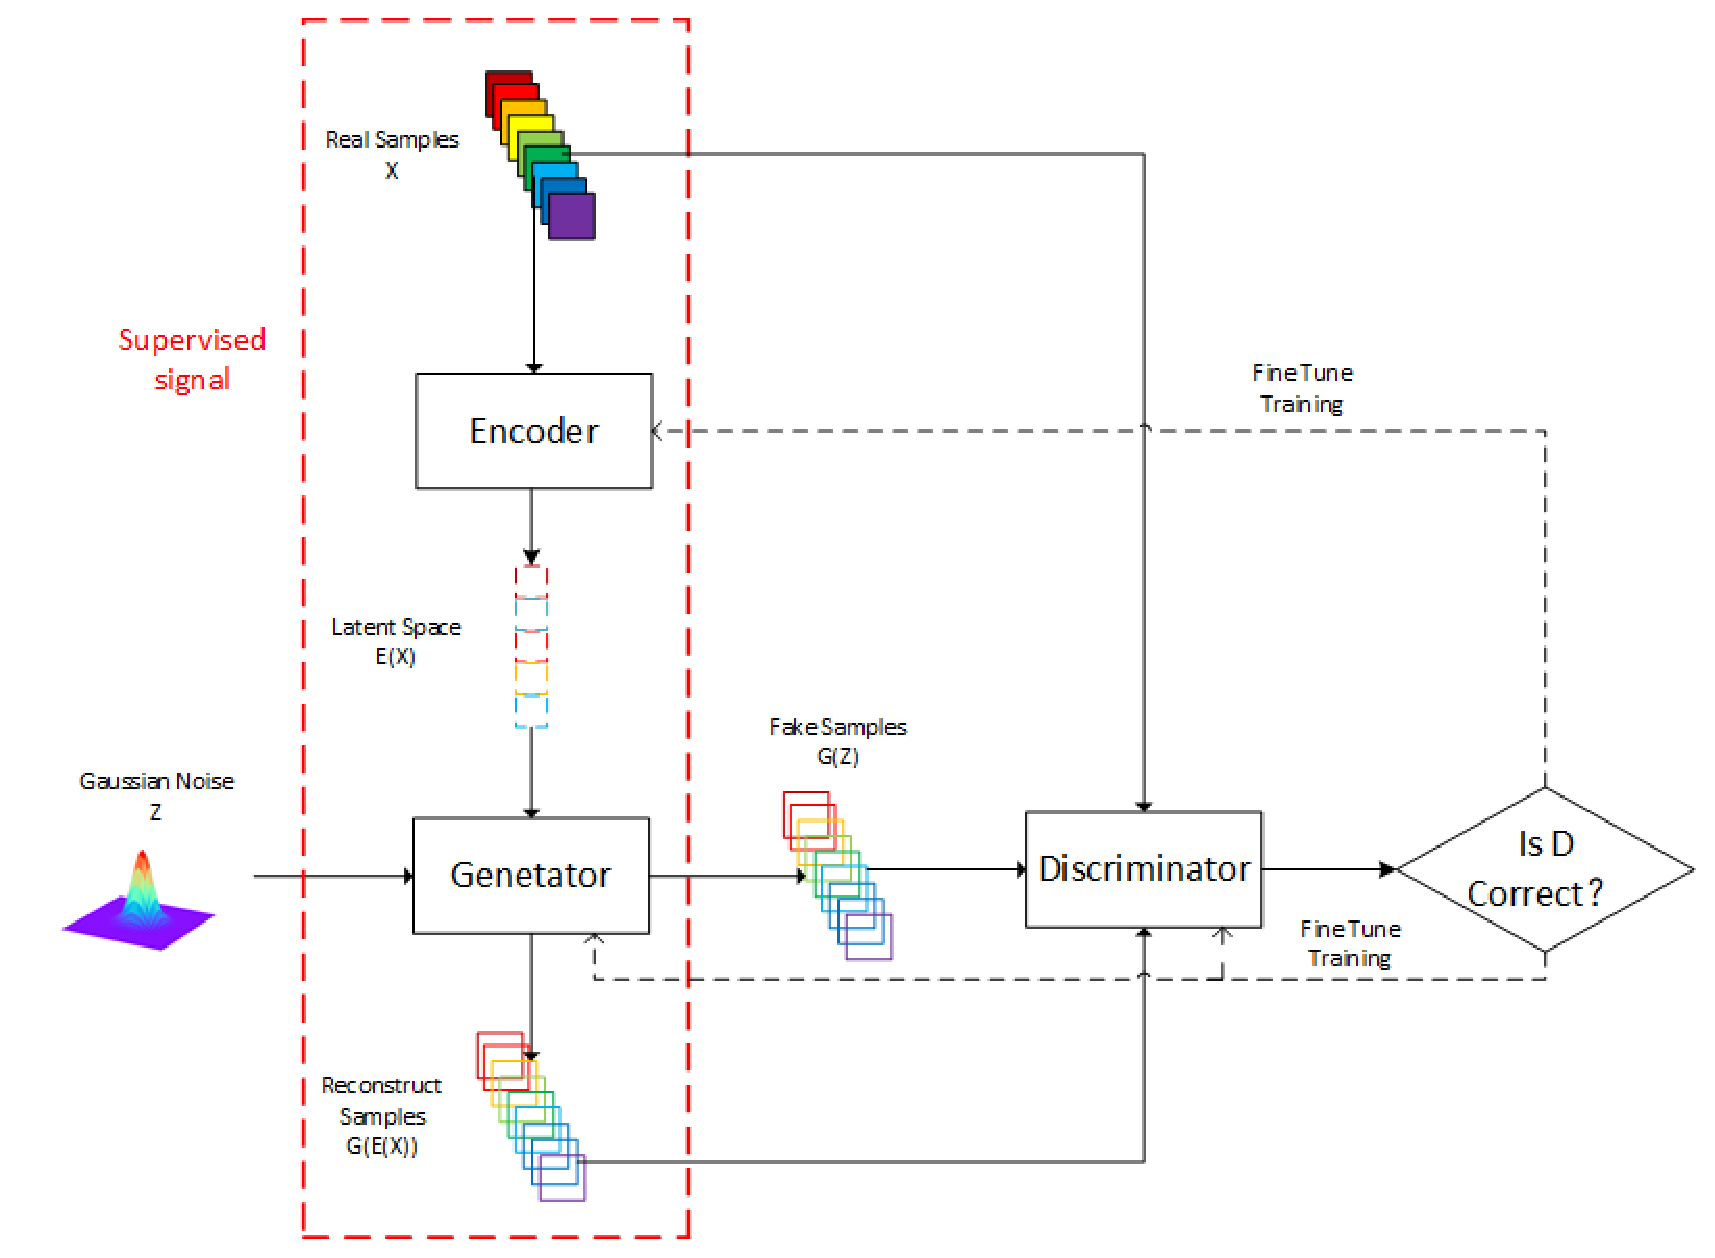
\includegraphics[width=\hsize]{example/2.eps}
	\bicaption[这里将出现在插图索引]
	{带监督信号的WGAN流程图}
	{Flowchart of WGAN with Supervised Signal}
	\label{fig2}
\end{figure}

图~\ref{fig2}中的所有样本都是一维非图像类数据集。可以看到除噪声数据外,还将自动编码机获得的隐向量数据表示形式输入到生成器中。生成器将隐藏变量转换为重构样本,优化的目标是期望重构样本尽可能接近真实样本。判别器通过最大限度地提高真样本和假样本的差异,从假样本、重构样本和真样本中获取信息。同时,生成器的目标是产生判别器无法区分的伪样本。判别器和生成器的训练过程是对抗性的。因为带监督信息的编码机能够遍历所有的原始样本,在原始数据中所有的分布都可以被模型学习到。有监督信号有助于学习到的概率密度函数能够均匀的分布在所有有原始样本的空间,从而为模态崩溃提供了有效的解决方案。这样生成的样本类型就不会过于单一。元素方向误差是在原有特征方向误差的基础上提高整体结构稳定性的一种方法。

在这里,编码器用于获取数据潜在的特征数据,通过最小化像素级别的误差 $ L ^ { 2 } $距离来提供更多信息:

\begin{equation}
\label{eq11}
T_{encoder} = D_{reconstruction}=\parallel X-G(E(X))\parallel^{2}
\end{equation}

这么做的好处是生成器可以将噪声样本$Z$和潜在样本$E(X)$分别转化为伪样本和重构样本,并从判别器那里获得较高的置信度系数。和原来的WGAN类似,这里我们仍旧使用Wasserstein距离作为统计标准来衡量两个数据分布的接近程度。这样经过引入了监督信号,新的算法优化目标函数变为:
\begin{equation}
\label{eq12}
T_{G} = -D(G(Z))-D(G(E(X)))+\parallel X-G(E(X))\parallel^{2}
\end{equation}

这里面$Z$ 是从简单的噪声分布中采样得到的数据,噪声的分布可以是均匀分布或者是高斯分布。对于判别器,$X$ 是真实的数据,因此应该能够得到较高的置信度。$G(Z)$ 和 $G(E(X))$都是假样本,应该从判别器那里得到比较低的打分值。这个过程的优化目标函数可以描述为:

\begin{equation}
\label{eq12}
T_{D} = D(X)-D(G(E(X)))-D(G(Z))
\end{equation}

整个算法的流程如下所示:

\begin{algorithm}[htpb]
	\caption{有监督信号的WGAN}% Ëã·¨±êÌâ
	\begin{algorithmic}[1]%Ò»ÐÐÒ»¸ö±êÐкÅ
		\Require ~~ \\
		对于生成器每次更新,判别器更新的次数$n_{critic}$,批训练样本大小$m$,训练迭代次数为 $K$.
		\For{$t=1$ to $K$}
		\For{$i=1$ to $n_{critic}$}
		\State 从噪声数据$Z$中采样$m$个数据:${z^{(1)},...,z^{(m)}}$
		\State 从真实数据$X$中采样$m$个数据:${x^{(1)},...,x^{(m)}}$ 
		\State 利用随机梯度上升法更新判别器网络参数:
		\begin{equation*}
		\nabla_{\theta_{d}}\frac{1}{m}\sum_{i=1}^m[D(x^{(i)})-\lambda {\rm{D(G(E(x^{(i)})))}}-D(G(z^{(i)}))]  
		\end{equation*}
		\EndFor
		\State 从噪声数据$Z$中采样$m$个数据:${z^{(1)},...,z^{(m)}}$
		\State 从真实数据$X$中采样$m$个数据:${x^{(1)},...,x^{(m)}}$
		\State 利用随机梯度下降法更新生成器网络参数:
		\begin{equation*}
		\nabla_{\theta_{d}}\frac{1}{m}\sum_{i=1}^m[-D(G(z^{(i)}))-\lambda {\rm{D(G(E(x^{(i)}))}}+\parallel x^{(i)}-G(E(x^{(i)})\parallel^{2}]
		\end{equation*}
		\State 利用随机梯度下降法更新自动编码器网络参数:
		\begin{equation*}
		\nabla_{\theta_{d}}\frac{1}{m}\sum_{i=1}^m[\parallel x^{(i)}-G(E(x^{(i)})\parallel^{2}]
		\end{equation*}
		\EndFor
	\end{algorithmic}
\end{algorithm}
\section{模型性能分析}
在本节将就改进模型的有效性和在标准数据集下不同参数中的表现进行分析,确定合理的参数方案。
\subsection{模型有效性分析}
由于数据的分布很难直观的观察到,为了可视化数据,首先生成一维概率密度分布已知的数据,从中采样得到相应的真实样本数据,把这些真实样本数据作为GAN网络的输入数据,然后绘制输出学习到的数据分布。观察生成数据和原始真实数据的吻合程度。

首先假设原始数据分布为两个高斯分布的叠加,第一个高斯分布为$\mu=4,\sigma=0.5$,第二个高斯分布为$\mu=0,\sigma=0.3$。原始数据分布形式如下:
\begin{figure}[!htp]
	\centering
	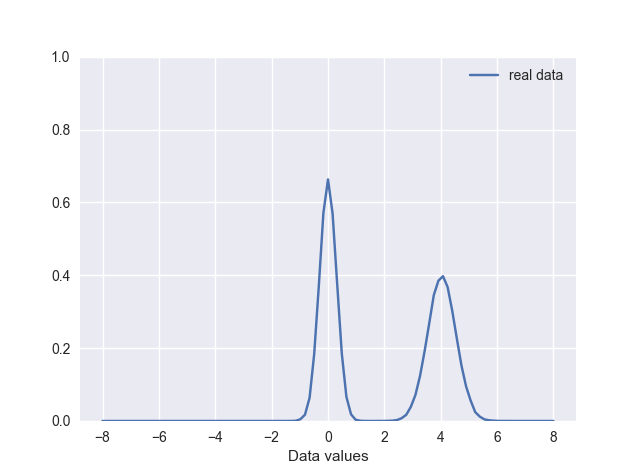
\includegraphics[width=\hsize]{example/yuanshi.png}
	\bicaption[这里将出现在插图索引]
	{原始高斯分布}
	{Flowchart of WGAN with Supervised Signal}
	\label{figyuanshi}
\end{figure}
对比WGAN,VAEGAN和改进的GAN算法,使用相同的网络结构,扩充数据量都为10000条,绘制扩充后的数据和原始数据的概率密度对比图如下:

\begin{figure}[!htp]
	\centering
	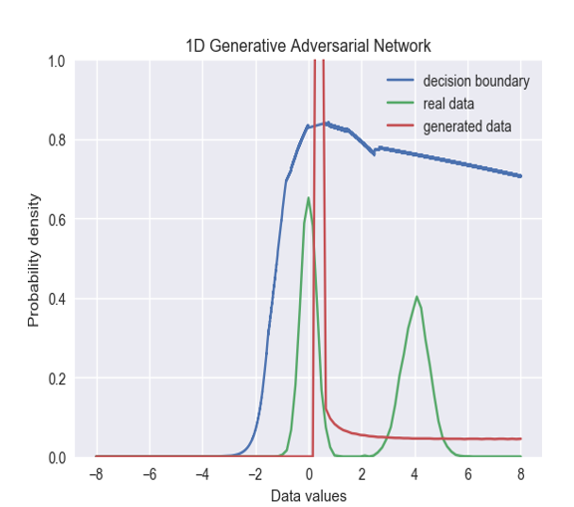
\includegraphics[width=10cm]{example/tu1.png}/
	\hspace{2cm}
	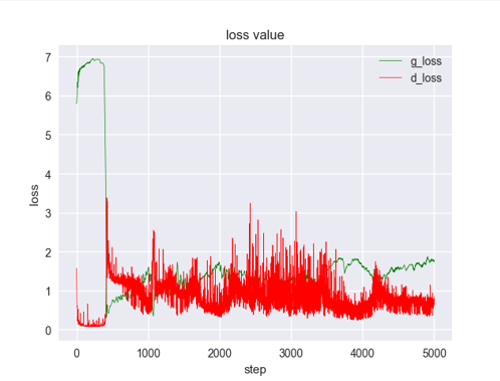
\includegraphics[width=10cm]{example/loss1.png}
	\bicaption[这里将出现在插图索引中]
	{WGAN 实验效果图}
	{Framework of GAN}
	\label{fig:al1}
\end{figure}
\begin{figure}[!htp]
	\centering
	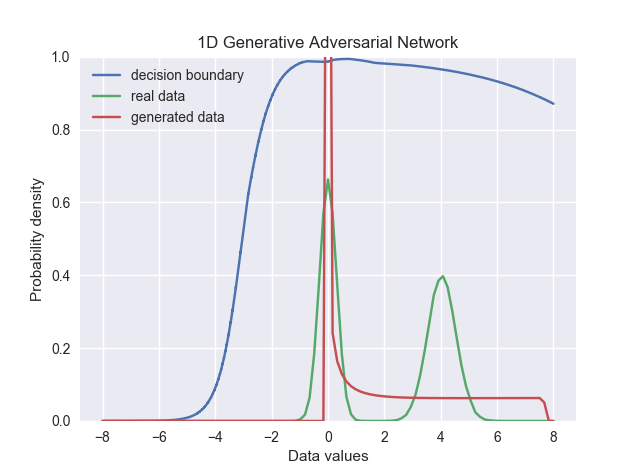
\includegraphics[width=10cm]{example/tu2.png}/
	\hspace{2cm}
	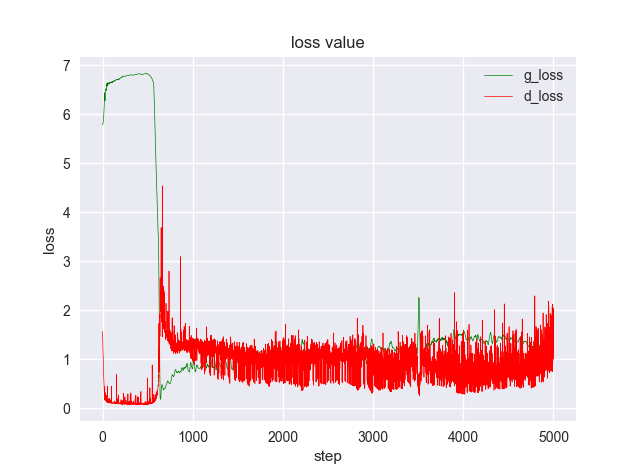
\includegraphics[width=10cm]{example/loss2.png}
	\bicaption[这里将出现在插图索引中]
	{VAEGAN实验效果图}
	{Framework of GAN}
	\label{fig:al2}
\end{figure}
\begin{figure}[!htp]
	\centering
	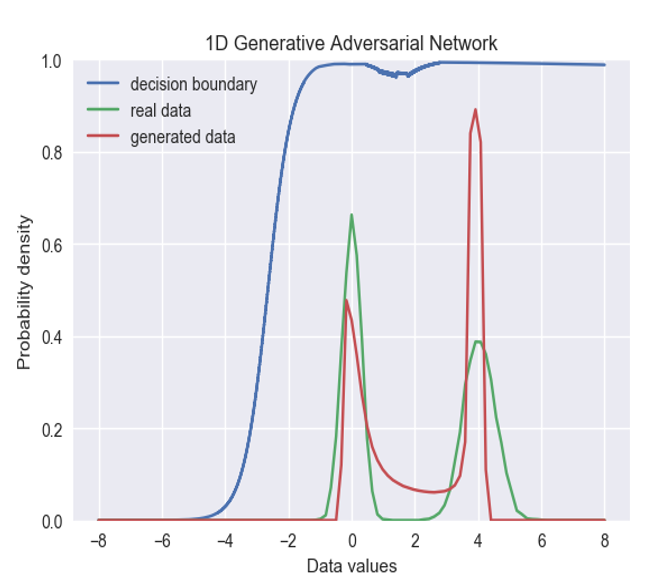
\includegraphics[width=10cm]{example/tu3.png}/
	\hspace{2cm}
	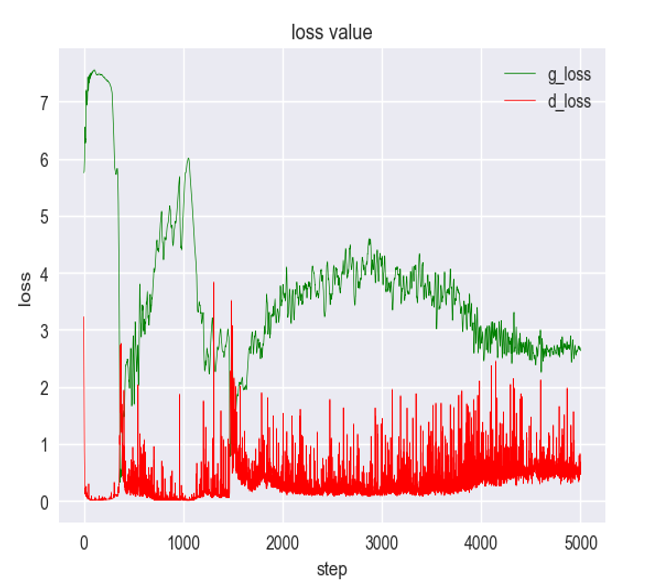
\includegraphics[width=10cm]{example/loss3.png}
	\bicaption[这里将出现在插图索引中]
	{改进WGAN实验效果图}
	{Framework of GAN}
	\label{fig:al3}
\end{figure}
可以看出,对于GAN算法,生成的数据只能学习到单高斯峰,而且生成的数据并不能准确描述$\mu=0,\sigma=0.3$的分布。判别器判别曲线还可能够判别出真假数据。从损失函数曲线上分析,两个网络始终没有达到相对稳定的状态。对于WGAN算法,仍然不能很好描述所有数据分布,但是由于引入了Wasserstein距离,损失函数曲线相比于GAN更加稳定,生成数据能相对准确的描述其中一个高斯分布,对于改进的WGAN算法,生成器已经能学到两个高斯分布,并且效果比前两种算法有所改善。对于损失函数生成器的损失函数大体呈下降趋势。通过对一维数据进行可视化,可以看出改进的算法在一定程度上改善了学习数据分布不全面,损失函数下降困难的问题。
\subsection{参数分析}
本节将结合标准数据集中联合循环发电厂(Combined Cycle Power Plant, CCPP)数据集讨论不同$\lambda$参数对实验结果带来的影响。该数据集包含了一个联合循环电厂在6年(2006-2011)的全负荷运行中收集到的9568个数据点。特征包括小时平均环境变量温度(T)、环境压力(AP)、相对湿度(RH)和排气真空(V),用于预测工厂的净小时电能输出(EP)。
数据集的描述如下:
\begin{table}[!hpb]
	\centering
	\caption{CCPP数据集描述}
	\label{tabccpp}
	\begin{tabular}{llll} \toprule
		属性名   & 描述 & 数据类型&数据范围  \\  \midrule
		Temperature&温度&浮点型(连续性)&$1.81^\circ C$, $37.11^\circ C$\\
		Ambient Pressure&环境压力&浮点型(连续性)&992.89, 1033.30 milibar\\
		Relative Humidity&相对湿度&浮点型(连续性)& 25.56$\%$, 100.16$\%$ \\
		Exhaust Vacuum&排气真空度&浮点型(连续性)&25.36, 81.56 cm Hg\\
		Hourly electrical energy output&每小时电能输出&浮点型(连续性)&420.26, 495.76 MW\\ \bottomrule
	\end{tabular}
\end{table}

原始数据量为9568个,用改进的WGAN算法扩充100000个,加入原始数据中观察数据扩充效果。设定生成数据量的大小都为选用的衡量指标是均方误差,通过设置不同$lambda$参数,平衡损失函数中数据生成和数据解码之间的关系。

为了评价新算法生成的样本质量,把所有数据归一化后,采用SVR模型进行回归,这里SVR使用径向基核函数。更多的拟合先验分布的伪样本可以改善回归结果。均值平方误差(Mean squared error, MSE)是一种反映SVR回归准确率的评价标准,用于间接检验数据增强实验的有效性。MSE的定义可以用公式\ref{eq14}表示:

\begin{equation}
\label{eq14}
MSE=\frac{\sum \limits_{i=1}^m (y^{i}-\bar{y})^{2}}{m}
\end{equation}

在这里 $y^{i}$ 是SVR预测的标签值,$\bar{y}$ 是原始数据的真实标签,测试数据集中有$m$样本,MSE值越小,误差越小,得到的生成样本越好。

图\ref{figCCPP}为CCPP数据集在不同$\lambda$参数下面的性能表现。
\begin{figure}[!htp]
	\centering
	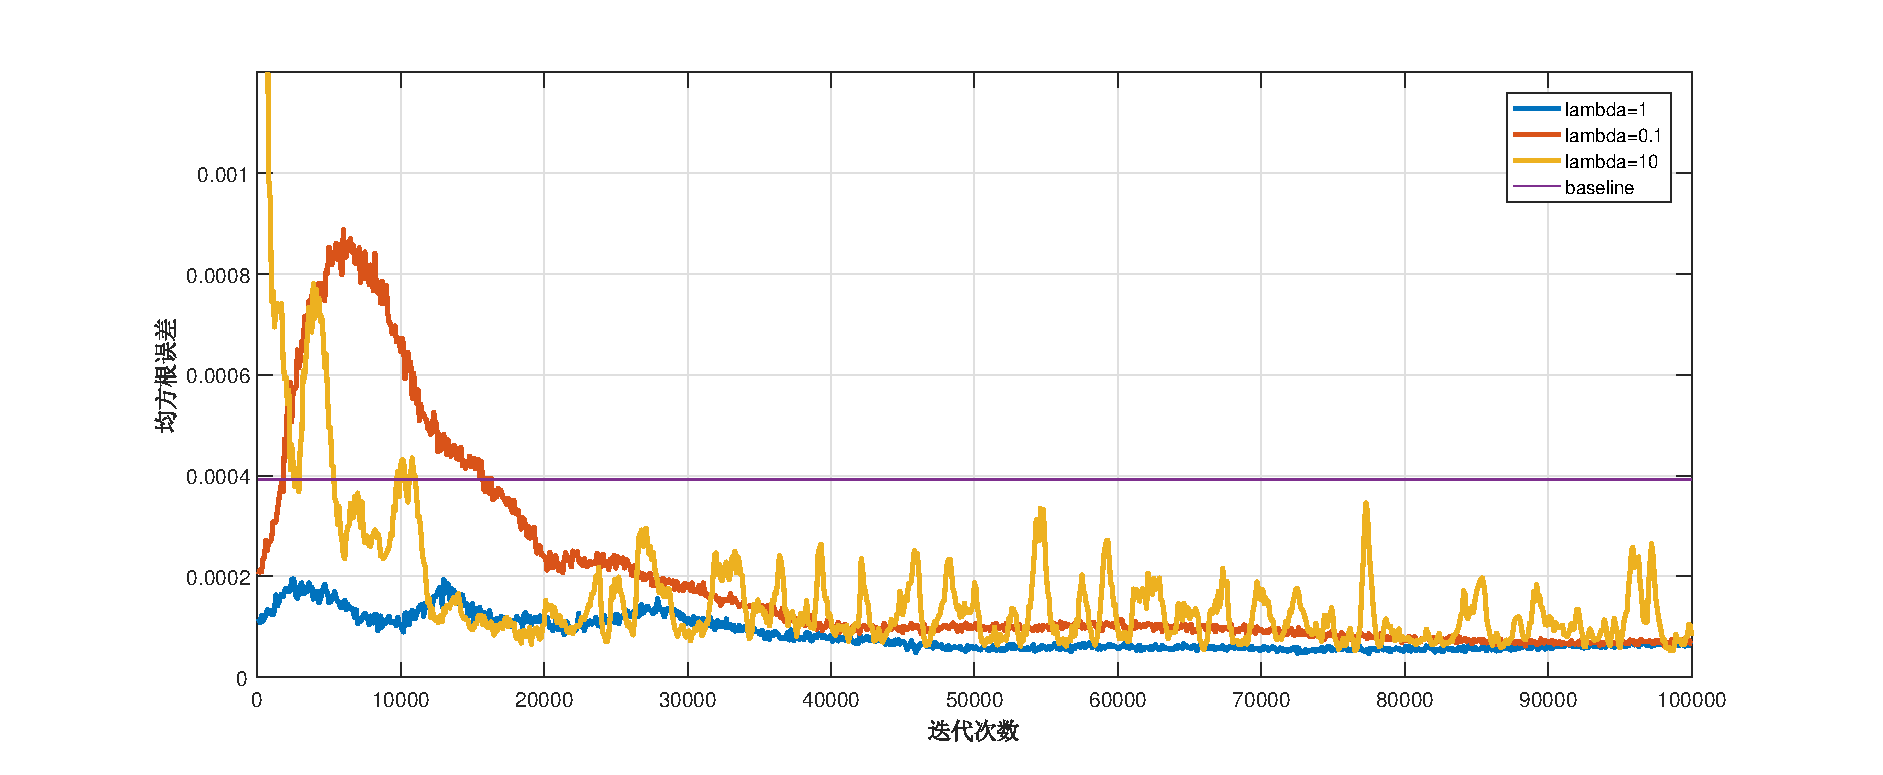
\includegraphics[width=\hsize]{example/CCPP.eps}
	\bicaption[这里将出现在插图索引]
	{CCPP数据实验结果}
	{Flowchart of WGAN with Supervised Signal}
	\label{figCCPP}
\end{figure}

可以看出,当$\lambda=10$时,改进的模型AE解码作用占比重相对较大,整个算法回归效果在前期并不理想,后期也存在严重的抖动问题。当$\lambda=0.1$,AE模型占比相对较小,无法知道GAN生成数据的方向,前期生成网络随机生成大量假样本,干扰了数据的质量,$\lambda=1$相对合理的平衡了生成模型和AE模型的权重,在网络的初始阶段曲线相对稳定,生成数据的质量相对较高,到后期随着迭代次数增加,MSE呈缓慢下降趋势。可以看出在迭代次数80000次后,曲线呈上升趋势,分析这是由于深度学习网络过拟合造成的,解决方案就是采用监控损失函数曲线,当发现loss呈上升趋势进行早停处理。


\section{实验结果及分析}
本节将给出实际的仿真结果和相应的结论。现有的GAN训练实验大多基于图像数据或视频数据。本文将改进后的新算法应用于一维数据的扩展。在这一部分,首先介绍评价数据扩充的标准,为了验证改进算法的可行性,分别对所测电子设备参数和5个指数股票序列数据集进行了实验,通过对比改进WGAN和传统算法进行数据扩充的结果进行分析。


在这里 $y^{i}$ 是SVR预测的标签值,$\bar{y}$ 是原始数据的真实标签,测试数据集中有$m$样本,MSE值越小,误差越小,得到的生成样本越好。

\subsection{电子设备参数实验}

本节数据集来自洛阳电子对抗基地。特征值的个数为10,输出响应变量为二维。另外,数据样本有72个,其中选择60个数据样本进行训练,选择12个样本进行测试。将改进算法应用于电子设备参数,验证了算法的稳定性。为了进行对照实验,也使用了VAEGAN和WGAN。对于编码器、解码器、生成器和判别器,所有对比模型都具有相同的架构。模型使用RMSProp优化算法进行训练,学习率为0.0003,批大小为24。表\ref{tab3}中列出了网络架构。

\begin{table}[hpb]
	\centering
	\caption{网络结构参数}
	\label{tab3}
	\begin{tabular}{lll} \toprule
		编码器   & 生成器 & 判别器  \\  \midrule
		12 fully-connected, ReLU &12 fully-connected, ReLU&12 fully-connected, ReLU\\
		24 fully-connected, ReLU&24 fully-connected, ReLU&24 fully-connected, ReLU\\
		24 fully-connected, None&24 fully-connected, ReLU&24 fully-connected, ReLU\\
		&12 fully-connected, None&1 fully-connected, None\\ \bottomrule
	\end{tabular}
\end{table}

训练迭代次数相同:选择60000次,生成的数据样本个数为25000个。通过生成的数据对测试数据进行回归,MSE值在迭代过程中发生变化,如图~\ref{fig3}所示。

\begin{figure}[htpb]
	\centering
	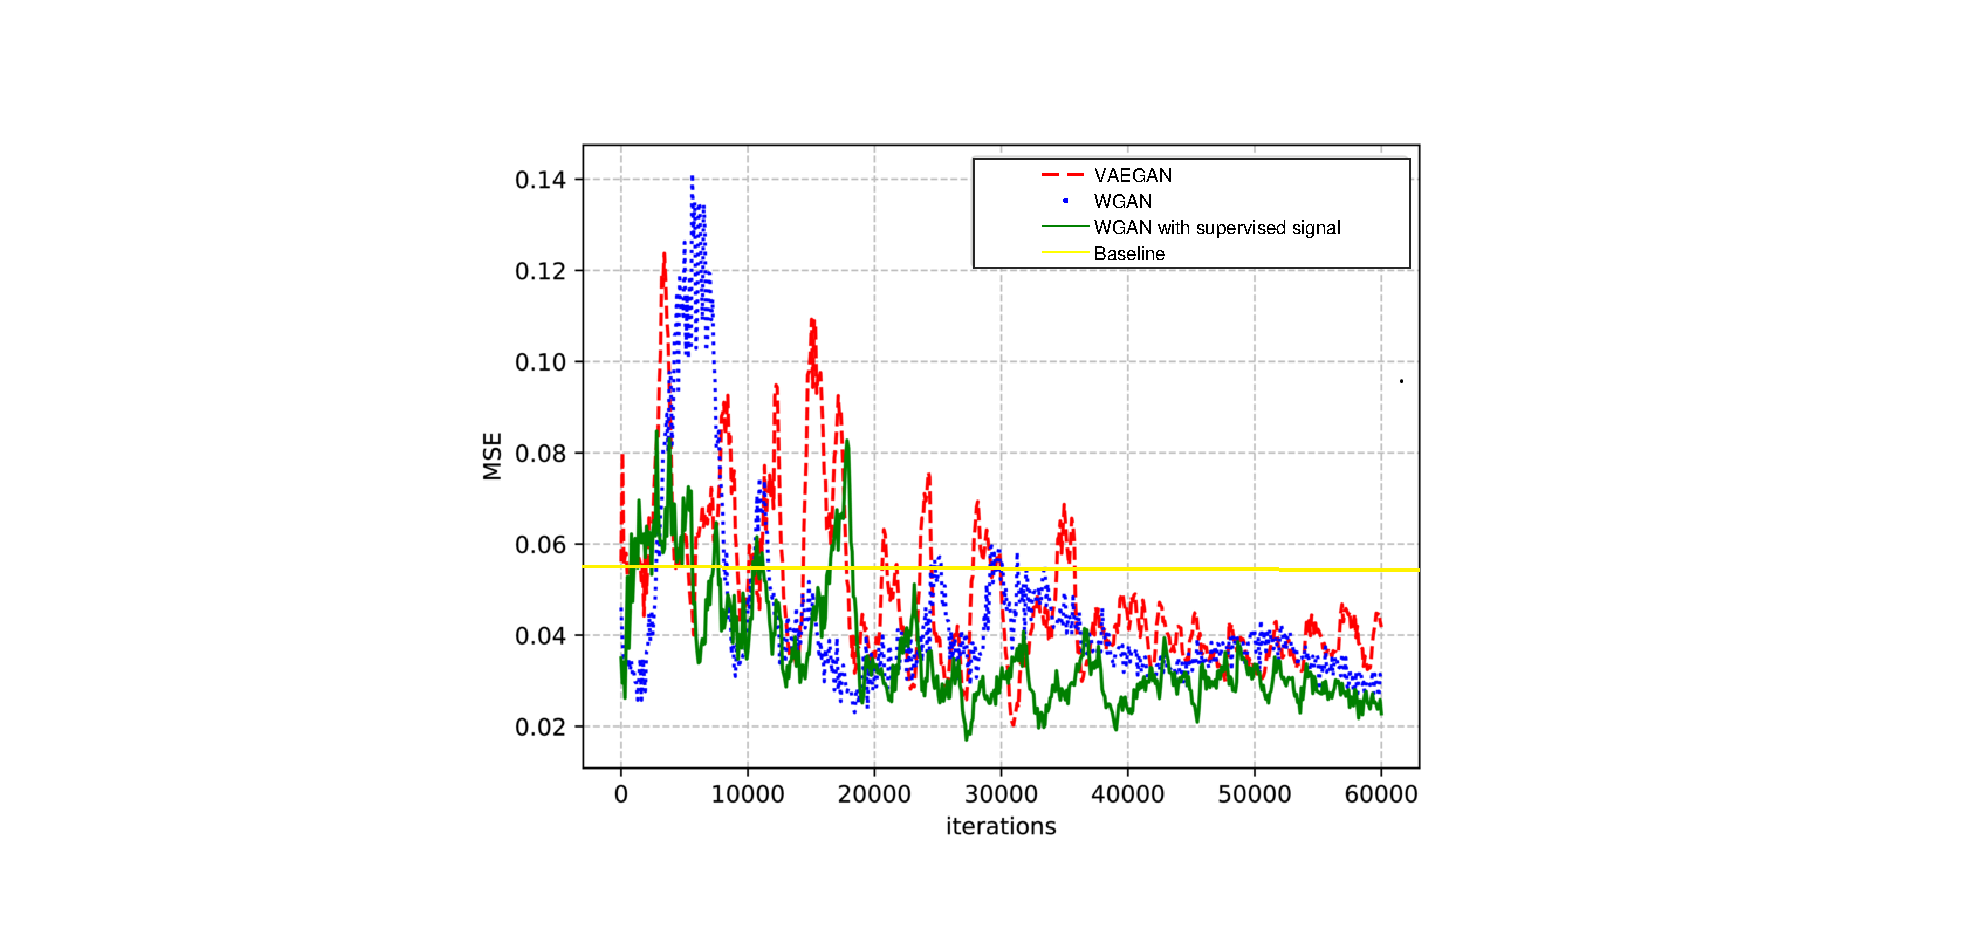
\includegraphics[width=\hsize]{example/GANsuanfaduibi.eps}
	\bicaption[这里将出现在插图索引]
	{不同模型生成数据进行回归MSE曲线图}
	{Mean squared error of different algorithms}
	\label{fig3}
\end{figure}

如图~\ref{fig3}所示,改进算法与VAEGAN和WGAN相比收敛速度更快,回归效果更好,反映了改进算法生成的样本更接近原始数据分布。在30000次迭代中,改进算法达到了稳定。由于有监督信号具有固定的先验分布,改进算法在训练初期的MSE明显低于其他算法。

\subsection{对于股票数据的回归}

为了消除实验的偶然性,我们分别对5个股票指数序列数据集进行了算法检验。与第4.1款设计的架构相同。表~\ref{tab1}给出了五种主要的股票价格指数,并使用了代码名。

\begin{table}[hpb]
	\centering
	\caption{股票数据详情}
	\label{tab1}
	\begin{tabular}{lll} \toprule
		股票价格指数   & 代码名称 &  数据区间  \\  \midrule
		All ordinaries   & AORD&  01/01/2016 to 01/09/2017 \\
		Dow Jones Industrial Average   & DJI&01/01/2016 to 01/09/2017\\
		Hang Seng Index   & HSI&   01/01/2016 to 01/09/2017\\
		KOSPI   & KS11& 01/01/2016 to 01/09/2017\\
		Nikkei Stock Average   &NK&   01/01/2016 to 01/09/2017\\
		\bottomrule
	\end{tabular}
\end{table}

这些数据来自雅虎财经网站\footnote{\url{https://finance.yahoo.com/}}。原始数据包括每天的开盘价、收盘价、最高价、最低价和成交量。选择增加收盘价。采用特征向量法\cite{18},利用最新的价格计算特征来处理序列数据。根据坐标延迟法,输入向量的维数为$m$,延迟时间为$d$,输入向量为$RDP_{1,d},…,RDP_ {m - 1 d}, EMA_{15}$和输出向量$RDP_ {d} $:

\begin{equation}
\label{eq16}
RDP_{i,d} = \frac{p(j)-p(j-i*d)}{p(j-i*d)}*100
\end{equation}


\begin{equation}
\label{eq17}
EMA_{15}  = p(j)-\bar{EMA_{15}(j)}
\end{equation}

\begin{equation}
\label{eq18}
RDP_{d} = \frac{\bar{p(j+d)}-\bar{p(j)}}{\bar{p(j)}}*100
\end{equation}


其中 $p(j)$ 是在时间点 $j$的价格。本文选择延迟时间$d=5$,输入向量维度$m=5$。分割前$80\% $的数据是训练数据,后$20\% $的数据是测试数据。分别利用VAEGAN、WGAN和我们算法对转换后的数据进行实验。回归结果如表\ref{tab2}:

\begin{table}[hpb]
	\centering
	\caption{股票数据回归结果}
	\label{tab2}
	\begin{tabular}{lllll} \toprule
		股票名称 & GAN &  VAEGAN & WGAN &Ours  \\ 
		\midrule
		AORD&0.01184 & 0.00667 & 0.00764 &\textbf{0.00622}   \\
		DJI &0.00816&0.00737&0.00769&\textbf{0.00643}  \\
		HSI&0.01762&0.01585&0.01612&\textbf{0.01409}  \\
		KS11&0.02655&0.02465&0.02621&\textbf{0.02413}\\
		NK & 0.07398& 0.03836& 0.04298&\textbf{0.03445} \\
		\bottomrule
	\end{tabular}
\end{table}

如表\ref{tab2}所示,利用带监督信号的WGAN实现非图像数据的增强是具有可行性的,对比于其他模型,表现出了更好的回归效果。本文提出的算法增加了有监督信号,该信号可以通过输入样本的潜在特征来约束生成器遍历所有真实样本。
改进后的算法有两个优点:
\begin{enumerate}
	\item 用自动编码机对数据编码的过程可以获得额外的学习知识,这使得生成器产生的伪样本很难被鉴别器识别。在有监督信号的情况下,生成的数据分布与之前的真实数据分布具有一对一的匹配关系,其对应关系保证生成的网络覆盖了真实数据的所有模式。
	\item 监督信号增强了WGAN输入的先验信息,避免了训练初期由于大量初始化参数而产生的随机样本,加快了训练过程,提升了生成样本的质量。
\end{enumerate}

\section{本章小结}

本章主要介绍了用强化学习模型进行数据增强的生成式对抗网络。在本章的第一部分介绍了GAN的背景意义,作为生成式模型的一种,GAN相对于传统的其他模型表现出了优良的性能。第二部分介绍了GAN的基本组成成为及算法的实现过程。GAN的生成器和判别器分别对应于强化学习Actor-Critic框架的Actor和Critic。在本章的第三部分介绍了GAN的优化算法WGAN,引入了Wasserstein距离的概念,并解释了为什么用Wasserstein来衡量数据分布的距离要优于其他度量参数。在本章的第四部分创新性的提出了引入监督信息的WGAN算法应用于非图像类数据的数据增强,其关键思想是在WGAN与编码器相结合时,通过输入样本的潜在特征来构造真实的样本。在描述改进算法的网络结构和优化的损失函数之后,文中给出了算法具体的实现过程。接着在文章的第五部分,针对改进的算法分别对实测的电子设备参数数据,和股票数据的回归问题上进行了实验,从理论上和实验上验证了新算法的可行性。

在训练初期,随着对原始参数的大量尝试的减少,改进的引入监督信息的WGAN收敛速度比其他两种算法都要快。新算法生成的数据更接近真实数据的分布。